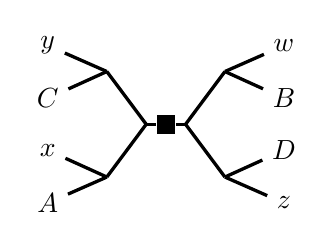
\begin{tikzpicture}
%\begin{scope}[every node/.style={circle,thick,draw}]
    \node (y) at (-1.5,1) {$y$};
    \node (C) at (-1.5,0.33) {$C$};
    \node (x) at (-1.5,-0.33) {$x$};
    \node (A) at (-1.5,-1) {$A$};
    
    \node (w) at (1.5,1) {$w$};
    \node (B) at (1.5,0.33) {$B$};
    \node (D) at (1.5,-0.33) {$D$};
    \node (z) at (1.5,-1) {$z$};
%\end{scope}
    \node (yC) at (-0.75, 0.67) {};
    \node (xA) at (-0.75, -0.67) {};
    \node (wB) at (0.75, 0.67) {};
    \node (zD) at (0.75, -0.67) {};
    
    \node (yCxA) at (-0.25, 0) {};
    \node (wBzD) at (0.25, 0) {};

\begin{scope}[every node/.style={fill=black,rectangle}]
    \node (root) at (0, 0) {};
\end{scope}
    
\begin{scope}[every node/.style={fill=white,circle},
              every edge/.style={draw=black,very thick}]
    \path [-] (y) edge (yC.center);
    \path [-] (C) edge (yC.center);
    \path [-] (x) edge (xA.center);
    \path [-] (A) edge (xA.center);
    \path [-] (w) edge (wB.center);
    \path [-] (B) edge (wB.center);
    \path [-] (z) edge (zD.center);
    \path [-] (D) edge (zD.center);
    
    \path [-] (yC.center) edge (yCxA.center);
    \path [-] (xA.center) edge (yCxA.center);
    \path [-] (wB.center) edge (wBzD.center);
    \path [-] (zD.center) edge (wBzD.center);
    
    \path [-] (yCxA.center) edge (root);
    \path [-] (wBzD.center) edge (root);
\end{scope}
\end{tikzpicture}